\documentclass[a4paper, 10pt]{article}
%\usepackage{fontspec}
%\setmainfont{Lato}
\usepackage{pgf}
\usepackage{eurosym}
\usepackage{graphicx}
\usepackage{wasysym}
\usepackage{hyperref}
\usepackage{listings}
\usepackage{pxfonts}
\usepackage{verbatim}
\usepackage{color}
\usepackage{xcolor}
\usepackage{wrapfig}
\usepackage{enumitem}
\usepackage{booktabs}
\usepackage{gensymb}
\usepackage{tabularx}
\usepackage{currfile}

\hypersetup{
    bookmarks=true,         % show bookmarks bar?
    unicode=true,          % non-Latin characters in Acrobat’s bookmarks
    pdftoolbar=true,        % show Acrobat’s toolbar?
    pdfmenubar=true,        % show Acrobat’s menu?
    pdffitwindow=true,     % window fit to page when opened
    pdftitle={Assessments},    % title
    pdfauthor={Paul Vesey},     % author
    pdfsubject={Advanced Graphics Assignment },   % subject of the document
    pdfcreator={},   % creator of the document
    pdfproducer={xelatex}, % producer of the document
    pdfkeywords={'Graphics' }, % list of keywords
    pdfnewwindow=true,      % links in new PDF window
    colorlinks=true,       % false: boxed links; true: colored links
    linkcolor=violet,          % color of internal links (change box color with linkbordercolor)
    citecolor=magenta,        % color of links to bibliography
    filecolor=red,      % color of file links
    urlcolor=blue           % color of external links
}

\setlength\parindent{0pt}
\begin{document}

\lstset{language=HTML,
				basicstyle=\small,
				breaklines=true,
        numbers=left,
        numberstyle=\tiny,
        showstringspaces=false,
        aboveskip=-20pt,
        frame=leftline
        }
				
\begin{table}%
	\begin{minipage}{0.4\textwidth}%
			
\includegraphics[width=1\textwidth]{./img/LITlogo.jpg}
	\end{minipage}
	\qquad
	\centering
	\parbox{0.4\textwidth}{
		\begin{large}			
			\begin{tabular}{| r | l |} \hline
				Subject: & \textbf{Advanced Graphics}\\
								 & \textbf{\& Visualisation}\\
				Course: & \textbf{Interior Design Y3}\\
				Session: & \textbf{Autumn 2020}\\
				Lecturer: & \textbf{Paul Vesey \footnotesize{BEng, MIE, HDip}}\\
				Filename: & \footnotesize{\currfilename}\\
				\hline
			\end{tabular}
		\end{large}			
	}
\end{table}
\vspace{0.25cm}	
	
\begin{flushleft}
\Large\textbf{Practical 1 - Practical Modeling }\\
\end{flushleft}

In this practical you are going to develop your modeling skills using a bitmap image template to assist in model creation.  Template files for 3DS have been created to get you started.  Select a model that is appropriate for your skill level.  You are advised to complete all three models over the coming weeks in order to hone your modeling skills.\\

The asset pack for this assignment can be downloaded from \href{https://goo.gl/EK5vwh}{https://goo.gl/EK5vwh}\\

You are not required to submit your completed models; they will not form part of your final grade in this subject.\\

\vspace{1cm}
\textbf{Easy}\\
\begin{figure}[hb]
	\centering
		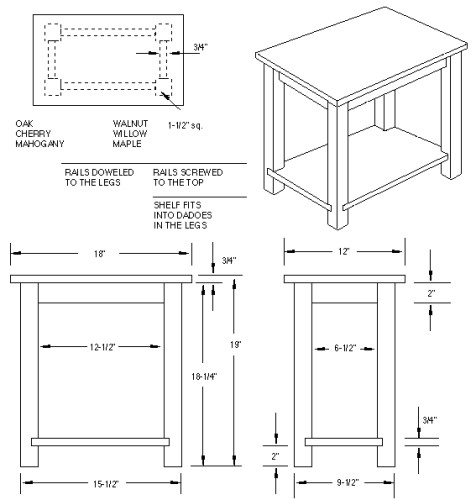
\includegraphics[width=6cm]{./img/wood-furniture-plans-1.jpg}
		\caption{Wood Table}
	\label{fig:Table}
\end{figure}


\newpage
\vspace{1cm}
\textbf{Moderate}\\
\begin{figure}[hb]
	\centering
		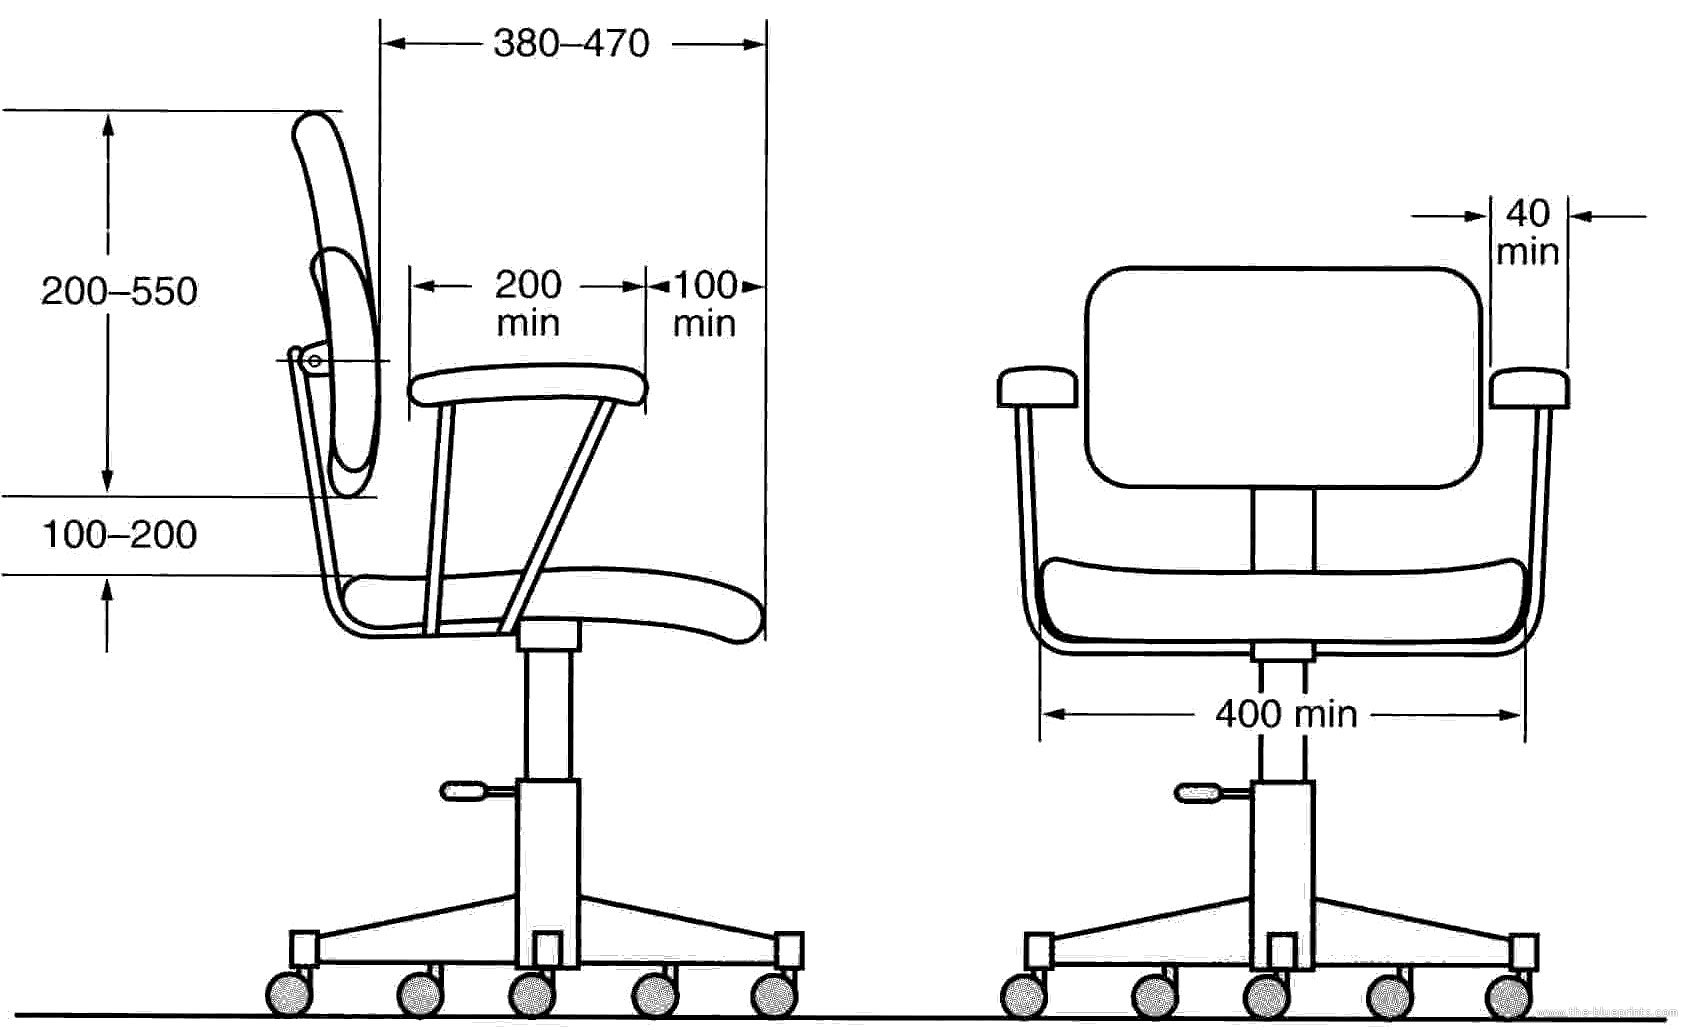
\includegraphics[width=6cm]{./img/office-chair-2.jpg}
		\caption{Office Chair}
	\label{fig:Office Chair}
\end{figure}


\vspace{1cm}
\textbf{Difficult}\\
\begin{figure}[hb]
	\centering
		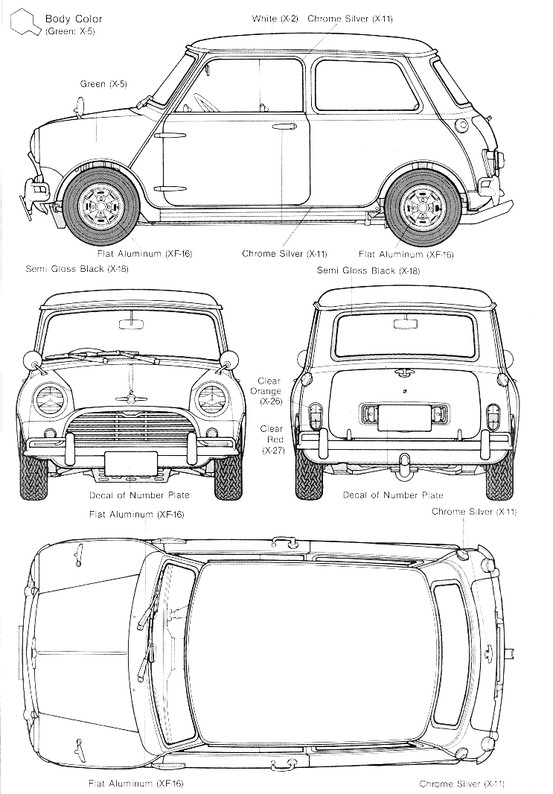
\includegraphics[width=6cm]{./img/mini.jpg}
		\caption{Austin Mini}
	\label{fig:Mini}
\end{figure}



\end{document}